\chapter{Display of VBF and Background-like Events}
 
\begin{figure}[H!]{16cm}
	\vspace{-20cm}
	\caption{Event display of the most VBF-like event ($H \rightarrow ZZ \rightarrow 2e2\mu$) according to the ANN in the \textbf{Njets2} category (ANN score = 0.93). As expected, the two jets present in the event have a very large $\eta$ separation and no particle activity between them.}
	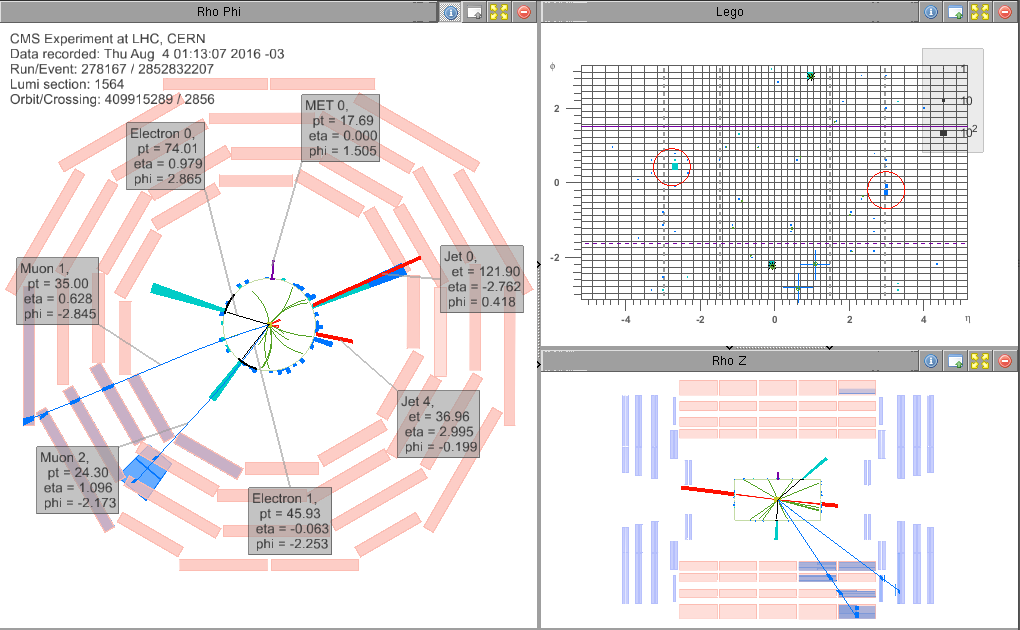
\includegraphics[scale=0.7,angle=90]{ChapterAnalysis/figs/event_display_Run278167_Lumi1564_Event2852832207_Njets2_ANN0p93_DoubleEG_Run2016F_2}
	\source{The AUTHOR, 2018.}
\end{figure}

\begin{figure}[H!]{16cm}
	\caption{Event display of the most background-like event ($H \rightarrow ZZ \rightarrow 4e$) according to the ANN in the \textbf{Njets2} category (ANN score = 0.04). Differing from the most VBF-like event, this one has the two jets very close in the $\eta-\phi$ space.}
	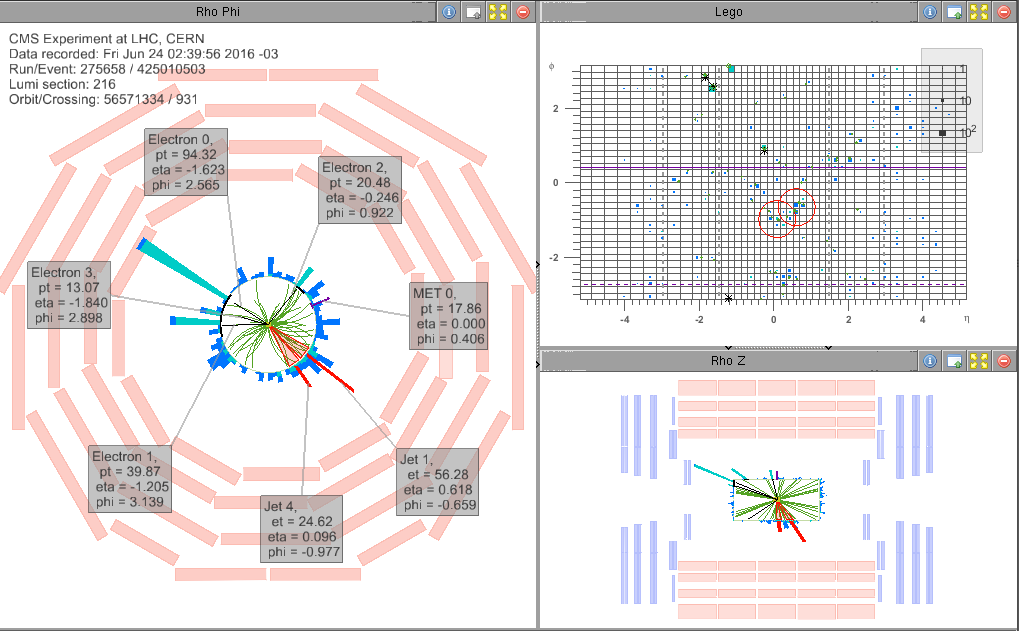
\includegraphics[scale=0.7,angle=90]{ChapterAnalysis/figs/event_display_Run275658_Lumi216_Event425010503_Njets2_ANN0p15_DoubleEG_Run2016C_2}
	\source{The AUTHOR, 2018.}
\end{figure}

\begin{figure}[H!]{16cm}
	\caption{Event display of the most VBF-like event ($H \rightarrow ZZ \rightarrow 4\mu$) according to the ANN in the \textbf{Njets3} category (ANN score = 0.77). By comparison, the $\eta$ gap between the jets and the particle activity is more evident than what is observed in the \textbf{Njets3} category for background (see next figure).}
	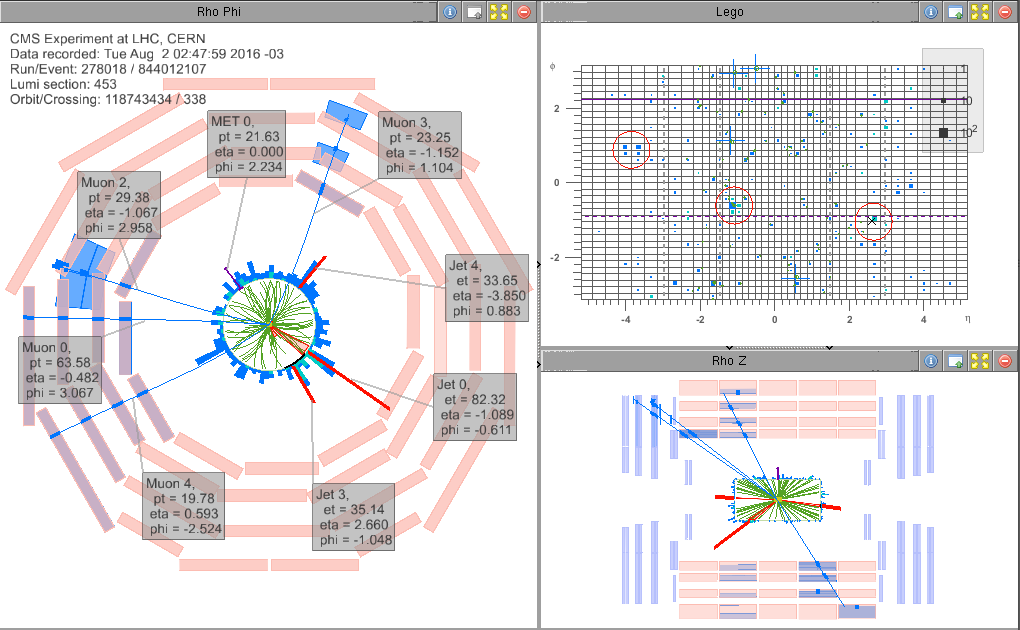
\includegraphics[scale=0.7,angle=90]{ChapterAnalysis/figs/event_display_Run278018_Lumi453_Event844012107_Njets3_ANN0p77_DoubleMuon_Run2016F_2}
	\source{The AUTHOR, 2018.}
\end{figure}

\begin{figure}[H!]{16cm}
	\caption{Event display of the most background-like event ($H \rightarrow ZZ \rightarrow 2e2\mu$) according to the ANN in the \textbf{Njets3} category (ANN score = 0.15).}
	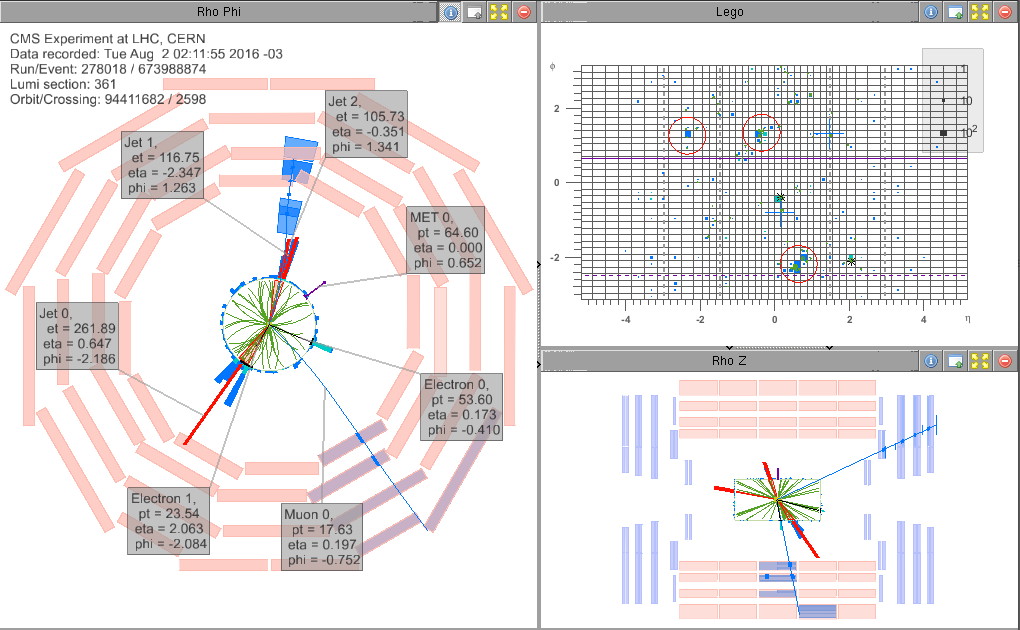
\includegraphics[scale=0.7,angle=90]{ChapterAnalysis/figs/event_display_Run278018_Lumi361_Event673988874_Njets3_ANN0p04_DoubleEG_Run2016F_2}
	\source{The AUTHOR, 2018.}
\end{figure}
	